\documentclass[dvipdfmx,11pt,a4paper,english,final]{article}

\usepackage[utf8]{inputenc}
\usepackage[OT1]{fontenc}
\usepackage{babel}

\usepackage[sfdefault,light]{roboto}
\renewcommand{\familydefault}{\sfdefault}
\usepackage{sfmath}
\usepackage{courier}
\usepackage{microtype}

\usepackage[breaklinks]{hyperref}
\usepackage[left=2cm,right=2cm,top=2.5cm,bottom=2.5cm]{geometry}

\usepackage{xcolor}
\usepackage{xspace}
\usepackage{multicol}
\usepackage{tikz}
\usetikzlibrary{%
  arrows.meta,%
  arrows,%
  backgrounds,%
  calc,%
  decorations.markings,%
  decorations.pathreplacing,%
  graphs,%
  matrix,%
  overlay-beamer-styles,%
  positioning,%
  shapes,%
}
\usepackage{adjustbox}

\newcommand{\ie}[0]{\textit{i.e.}\xspace}
\newcommand{\etc}[0]{\textit{etc.}\xspace}
\newcommand{\afortiori}[0]{\textit{a~fortiori}\xspace}


\newcommand{\gp}[0]{Glo\-bal\-Plat\-form\xspace}


\newcommand{\cardks}[0]{\ensuremath{\mathrm{K}_\mathrm{card}^s}\xspace}
\newcommand{\cardkp}[0]{\ensuremath{\mathrm{K}_\mathrm{card}^p}\xspace}
\newcommand{\cardcert}[0]{\ensuremath{\mathrm{Cert}_\mathrm{card}}\xspace}

\newcommand{\cardeks}[0]{\ensuremath{\mathrm{eK}_\mathrm{card}^s}\xspace}
\newcommand{\cardekp}[0]{\ensuremath{\mathrm{eK}_\mathrm{card}^p}\xspace}
\newcommand{\oceeks}[0]{\ensuremath{\mathrm{eK}_\mathrm{OCE}^s}\xspace}
\newcommand{\oceekp}[0]{\ensuremath{\mathrm{eK}_\mathrm{OCE}^p}\xspace}

\newcommand{\shse}[0]{\ensuremath{\mathrm{ShSe}}\xspace}
\newcommand{\shss}[0]{\ensuremath{\mathrm{ShSs}}\xspace}


\newcommand{\code}[1]{\texttt{#1}\xspace}
\newcommand{\todo}[1]{\textbf{\textcolor{red}{#1}}\xspace}



\title{Secure messaging for OpenPGP card version 3.x}

\begin{document}

\maketitle

\section*{Introduction}

OpenPGP card specification\cite{openpgp-card} defines a mean to ensure
integrity and confidentiality of communications with the OpenPGP card
application. This concept, called \emph{secure messaging}, is well
known and widely used in the smart card ecosystem~\cite{iso7816-4,
  gp-card}. However, the secure messaging defined in OpenPGP card
specification is not as secure as other secure messaging protocols
such as \emph{Secure Channel Protocols (SCP)} from \gp
specifications, and is not intented to protect communications
\emph{only}.

The most severe issue with secure messaging of OpenPGP card is the
mutual authentication between an off card entity (OCE) (\ie
computer, smartphone, \etc) and a OpenPGP card based on static AES
keys. If these keys get compromised, forward secrecy of communications
is not ensured, and man-in-the-middle attacks are easily
practicable. Moreover, this scheme is not convenient to use in
practice.  For a card with no keys set, the OCE can generates such
keys and store them in the card by transmitting them in clear after
correct verification of PW3 (admin PIN), also transmitted in
clear. For a card with some keys set, the OCE must also know them a
priori in order to use them for secure messaging.  However, it means
that these keys exist on each OCE, and so for each card, assuming that
each card has its own keys. Both cases are neither practicable nor
secure.

In addition to the problem of using static keys, the secure lessaging
feature described in OpenPGP card specification imposes to use a new
initialization vector (IV) generated by the card between each
command/response. Concretely, before each command that needs to be
protected the OCE must ask the card for a fresh IV (\afortiori
transmitted in clear), which adds a strong overhead in terms of
communications with the card.

Finally, the OpenPGP card specification says that a command protected
with secure messaging as the same level of privileges that a
non-protected command executed after successful presentation of PW3
(admin PIN), including the ability to reset the try counter of PW1
(user PIN), to override existing PGP keys and certificates, but also
to set static keys for secure messaging. Since secure messaging grants
admin privileges, it cannot be used to protect integrity and
confidentiality of commands/responses only.

For these reasons, the secure messaging feature of OpenPGP
specification is more an alternative way of administrating a card to
the traditional verification of PW3 (admin PIN) than a mean to protect
communications with an OpenPGP card. In this document, we propose to
replace the existing secure messaging feature of OpenPGP card
specification by a state-of-the-art secure messaging feature to
protect communications with a card only. Basically, we propose to
reuse an existing \emph{Secure Channel Protocol (SCP)} from \gp
specifications with as few modifications as possible to be used with
the current OpenPGP card specification.


\section{Secure Channel Protocol}
\label{sec:scp}

\gp specifies several secure channel protocols with variable security
guarantees. Most of these protocols provide a mutual authentication
between a card and an OCE based on a shared secret such as a set of
static DES (SCP01 and SCP02) or AES (SCP03) keys. Relying on a shared
secret is not convenient in practice as it requires to spread this
secret among all OCEs, and so for each card. The only secure channel
procotol specified by \gp not relying on a shared secret is the SCP11.

\subsection{SCP11 overview}

Two variants of SCP11 exist: SCP11a which allows mutual authentication
of an OCE and a card, and SCP11b which handles only card
authentication by an OCE.

The authentication of an OCE by a card in SCP11a requires that each
OCE as its own certificate that each card can accept directly and/or
can verify it according to a known certification authority. This
scheme is not convenient in the context of a OpenPGP card as it
requires to deploy a certificate and its corresponding private key on
each OCE. Then, it is not better than SCP11b in terms of security in
our context. Actually, as SCP11a contains no revocation mechanism, it
is equivalent to not having OCE authentication as soon as an
``entity'' is compromised.

For these reasons, SCP11b is a good compromise for OpenPGP. The static
private key embedded in an card is as secure as other OpenPGP keys it
already handles, and it is possible to generate this key on board. The
security of the protocol thus relies only on protection of the private
key of the certification authority that is signing the card’s
certificate, and in the integrity of this certificate on OCEs.

\subsection{Details of SCP11b}

The specification of SCP11b is splitted in several
documents~\cite{gp-scp03, gp-upgrade, gp-scp11} as it involves
mechanisms from other secure channel protocols defined by \gp. The key
agreement protocol used in SCP11b~\cite{gp-scp11}, which is specific
to SCP11, is a variant of the ElGamal key agreement protocol. On the
contrary, the secure messaging part of SCP11 is exactly the one used
in SCP03~\cite{gp-scp03}. It involves AES in CBC mode for
command and response encryption, and CMAC~\cite{nist-cmac} with AES for
command and response integrity.

Figure~\ref{fig:scp11} depicts the key agreement part of SCP11b with
notations detailed in table~\ref{tab:notations} (section~5.1
in~\cite{gp-scp11}). All keypairs denoted in figure~\ref{fig:scp11} use the same
elliptic curve. In practice, the this curve is implicit known by both
entities as it is the elliptic curve used for the static keypair
(\cardks, \cardkp) of the card. This curve also detemines the size of
AES keys (section~5.2 in~\cite{gp-scp11}) for the secure messaging
part: if size of an EC point on the curve is strictly lower than 512
bits, then generated session AES keys must be 128 bits long, otherwise
these keys must be 256 bits long.

\begin{table}[ht]
  \centering
  \begin{tabular}{|l|l|}
    \hline
    \cardks&Static private key of the card\\
    \cardkp&Static public key of the card\\
    \cardcert&Certificate corresponding to the keypair (\cardks, \cardkp)\\
    \hline
    \oceeks&Ephemeral private key of the OCE\\
    \oceekp&Ephemeral public key of the OCE\\
    \cardeks&Ephemeral private key of the card\\
    \cardekp&Ephemeral public key of the card\\
    \hline
    \shss&Shared secret generated involving the static key of the card\\
    \shse&Shared secret generated involving only ephemeral keys\\
    \hline
  \end{tabular}
  \caption{Notations for keys and secrets involved in SCP11b.}
  \label{tab:notations}
\end{table}

\begin{figure}[ht]
  \centering
  \begin{adjustbox}{fbox,max size={.98\textwidth}{.9\textheight}}
    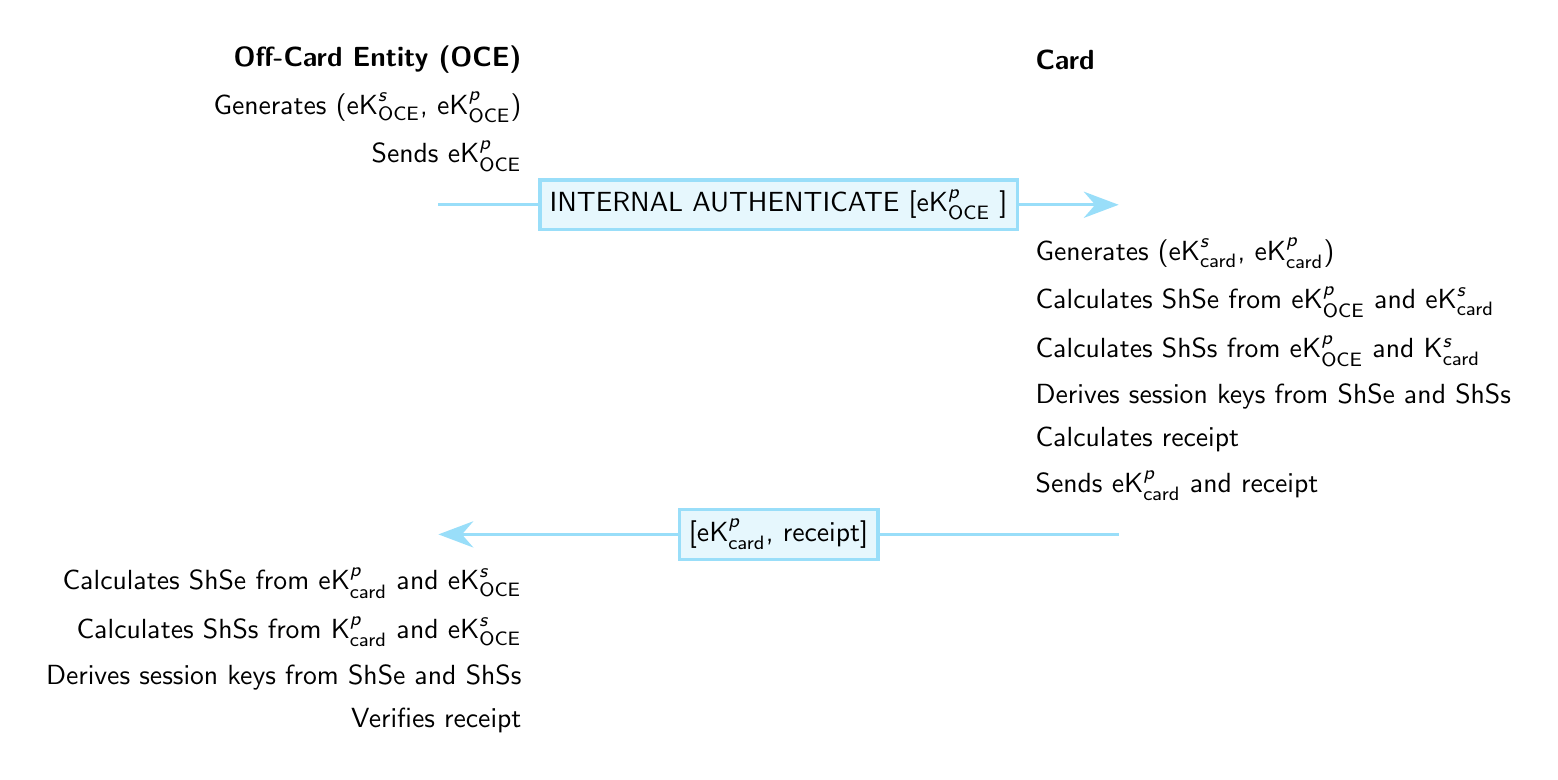
\begin{tikzpicture}[%
      oce/.style={anchor=east},%
      card/.style={anchor=west},%
      msg/.style={anchor=center},%
      diag/.style={draw=cyan!40, very thick, fill=cyan!10},%
      arr/.style={draw=cyan!40, very thick, fill=cyan!40},%
      ]
      
      \matrix (mat) [%
      matrix of nodes,%
      nodes in empty cells,%
      ] %,row sep=3em,column sep=4em,]
      {
        |[oce]| {\textbf{Off-Card Entity (OCE)}}&&|[card]| {\textbf{Card}}\\
        |[oce]| {Generates (\oceeks, \oceekp)}&&\\
        |[oce]| {Sends \oceekp}&&\\
        &|[msg]| {INTERNAL AUTHENTICATE [\oceekp]}&\\
        &&|[card]| {Generates (\cardeks, \cardekp)}\\
        &&|[card]| {Calculates \shse from \oceekp and \cardeks}\\
        &&|[card]| {Calculates \shss from \oceekp and \cardks}\\
        &&|[card]| {Derives session keys from \shse and \shss}\\
        &&|[card]| {Calculates receipt}\\
        &&|[card]| {Sends \cardekp and receipt}\\
        &|[msg]| {[\cardekp, receipt]}&\\
        |[oce]| {Calculates \shse from \cardekp and \oceeks}&&\\
        |[oce]| {Calculates \shss from \cardkp and \oceeks}&&\\
        |[oce]| {Derives session keys from \shse and \shss}&&\\
        |[oce]| {Verifies receipt}&&\\
      };

      \scoped[on background layer]{%
        \path[arr] ($(mat-4-1.west) - (3em,0)$) edge[-{Stealth[scale=1.5]}] ($(mat-4-3.east) + (3em, 0)$);
        \path[arr] ($(mat-11-1.west) - (3em,0)$) edge[{Stealth[scale=1.5]}-] ($(mat-11-3.east) + (3em,0)$);
        
        \path[diag] (mat-4-2.north west) rectangle (mat-4-2.south east);
        \path[diag] (mat-11-2.north west) rectangle (mat-11-2.south east);
      }
      \end{tikzpicture}
    \end{adjustbox}
  \caption{SCP11b key agreement.}
  \label{fig:scp11}
\end{figure}




\section{Specification of SCP11b for OpenPGP card}

The commands from SCP11b specification cannot be integrated as is in
OpenPGP specification: some commands required for SCP11b already exist
with a different meaning in OpenPGP card specification, some
parameters of these commands have no meaning in our context, or some
parameters have been specified differently in SCP11b and in OpenPGP
card specification.

To implement SCP11b, the following actions are required:
\begin{itemize}
\item to store an authentication certificate and the corresponding
  private key in a card;
\item to request a card for its authentication certificate and the
  corresponding public key;
\item to initialize a secure messaging session, \ie authenticate a
  card and establish session keys as depicted in
  figure~\ref{fig:scp11}.
\end{itemize}

Each of these actions can be implemented by an APDU command (section~6
in~\cite{gp-scp11}), as described in
sections~\ref{sec:card-provisionning} and~\ref{sec:authentication} of
this document.

The secure messaging part of SCP11b, that is encryption/decryption and
MAC computation/verifi- cation of commands and responses, does not
require specific commands. The signalisation bit(s) in the CLA byte of
commands protected by secure messaging differs between \gp
and OpenPGP specifications. In order not to interfere with existing
implementations using the secure messaging feature of OpenPGP cards,
the CLA byte is altered as described in section~\ref{sec:sm}.

\subsection{Card provisioning}
\label{sec:card-provisionning}

While the certificate \cardcert must be generated and signed out of
the card, the corresponding keypair (\cardks, \cardkp) can either be
generated out of the card and then imported in the card, or generated
by the card itself. The generation of the certificate and its
signature by a trusted entity is out of the scope of this
document. However, it is important to note that if the keypair is
generated out of the card, it must be an EC keypair for a curve
supported by OpenPGP specification.

The table~\ref{tab:scp11:descriptors} gives the new descriptors
introduced in OpenPGP card specification to denote the new objects
required for SCP11b implementation. These descriptors permit to handle
the corresponding objects as other objects of the same kind (\ie
keypairs, certificates) in OpenPGP card specification (sections~4.4.1
and 4.4.2 in~\cite{openpgp-card}). Each key is assigned a
\emph{Control Reference Template (CRT)} (section~4.4.3.9
in~\cite{openpgp-card}) and some algorithm attributes (section~4.4.3.7
in~\cite{openpgp-card}). The CRT \code{A600} (section~6.2
in~\cite{gp-scp11}) is used to reference the card authentication
static keypair (\cardks, \cardkp), and the tag \code{D4} for the
corresponding algorithm attributes. The card authentication
certificate \cardcert corresponding to this keypair is referenced by
% the tag \code{7F21} as the fourth occurrence.
the tag \code{FB}.

\begin{table}[ht]
  \centering
  \begin{tabular}{|l|l|}
    \hline
    \code{A600}&Control reference template (CRT) for the card static keypair (\cardks, \cardkp)\\
    \code{D4}&Tag for the algorithm attributes of the card static keypair (\cardks, \cardkp)\\
    \hline
  \end{tabular}
  \caption{New descriptors for SPC11b implementation in OpenPGP card specification.}
  \label{tab:scp11:descriptors}
\end{table}



\subsubsection{Setting algorithm attributes for (\cardks, \cardkp)}

Before a keypair is generated or imported, the corresponding algorithm
attributes must be set. The algorithm attributes for the keypair
(\cardks, \cardkp) are set via the PUT DATA command with INS=\code{DA} and
P1P2=\code{D4} (section~7.2.8 in~\cite{openpgp-card}). The algorithm attributes for this
keypair must be valid ECDH attributes (section~4.4.3.7 in~\cite{openpgp-card}),
otherwise the card must issue an error and must not modify existing
values.

\subsubsection{Generating/importing (\cardks, \cardkp)}

The card authentication keypair can be generated via the GENERATE
ASYMMETRIC KEY PAIR command with P1=\code{80} and the data field set
to \code{A600} (section~7.2.13 in~\cite{openpgp-card}). If the command
exits normally, the public key of the generated keypair is returned
(see section~\ref{sec:read:cardkp}).

The card authentication keypair can be
imported via the PUT DATA command with INS=\code{DB}, P1=\code{3F},
P2=\code{FF} and the data field set to the extended header list for
ECDH with CRT set to \code{A600} (sections~4.4.3.9 and 7.2.8
in~\cite{openpgp-card}).

\subsubsection{Importing \cardcert into the card}

% The card authentication certificate \cardcert can be imported via a
% sequence of two commands:
% \begin{enumerate}
% \item SELECT DATA with P1=\code{03}, P2=\code{04} and the data field
%   set to \code{60045C027F21} (section~7.2.5 in~\cite{openpgp-card});
% \item PUT DATA with INS=\code{DA} and P1P2=\code{7F21} (section~7.2.8
%   in~\cite{openpgp-card}).
% \end{enumerate}

% The first command selects the fourth occurrence for the tag \code{7F21},
% which is used to identify certificates. The second command actually
% imports the certificate.

The card authentication certificate \cardcert can be imported via a
PUT DATA with INS=\code{DA} and P1P2=\code{00FB} (section~7.2.8
in~\cite{openpgp-card}).


\subsubsection{Reading \cardcert from the card}

% The card authentication certificate \cardcert can be retrieved at any
% time via a sequence of two commands:
% \begin{enumerate}
% \item SELECT DATA with P1=\code{03}, P2=\code{04} and the data field set to \code{60045C027F21} (section~7.2.5 in~\cite{openpgp-card});
% \item GET DATA with P1P2=\code{7F21} (section~7.2.6 in~\cite{openpgp-card}).  
% \end{enumerate}

% The first command selects the fourth occurrence for the tag \code{7F21},
% which is used to identify certificates. The second command actually
% reads the certificate.

The card authentication certificate \cardcert can be retrieved at any
time via a GET DATA with P1P2=\code{00FB} (section~7.2.6
in~\cite{openpgp-card}).


\subsubsection{Reading only \cardkp from the card}
\label{sec:read:cardkp}

The card authentication public key \cardkp can be retrieved at any
time via the GENERATE ASYMMETRIC KEY PAIR command with P1=\code{81} and the
data field set to \code{A600} (section~7.2.13 in~\cite{openpgp-card}).

\subsection{Authentication and key agreement}
\label{sec:authentication}

The INTERNAL AUTHENTICATE is already specified in the OpenPGP card
specification (section~7.2.12 in~\cite{openpgp-card}), but for another
purpose, when P1 = P2 = \code{0}. Since this is the only behavior
described in the specification, other values of P1 and P2 can be used
to implement the key agreement part of SCP11b depicted in section~\ref{sec:scp}.

On the contrary to the existing INTERNAL AUTHENTICATE command with
P1P2=\code{0000}, this INTERNAL AUTHENTICATE command does not require the
verification of PW2 (user PIN for signature).

The authentication and key agreement is achieved by issuing the
INTERNAL AUTHENTICATE command with P1P2=\code{0100} and the data field
set to the content depicted in table~\ref{tab:scp11:auth:cmd} (section
6.5.2.3 in~\cite{gp-scp11}).

\begin{table}[ht]
  \centering
  \begin{tabular}{|c|c|ccl|}
    \hline
    \textbf{Tag}&\textbf{Length}&\multicolumn{3}{l|}{\textbf{Value description}}\\
    \hline
    \code{A6}&13&\multicolumn{3}{l|}{Control reference template}\\
    \cline{3-5}
                &&\multicolumn{1}{c|}{\textbf{Tag}}&\multicolumn{1}{c|}{\textbf{Length}}&\textbf{Value description}\\
    \cline{3-5}
                &&\multicolumn{1}{c|}{\code{90}}&\multicolumn{1}{c|}{2}&\code{1100} (SCP11b without IDs)\\
                &&\multicolumn{1}{c|}{\code{95}}&\multicolumn{1}{c|}{1}&\code{3C} (MAC + encryption)\\
                &&\multicolumn{1}{c|}{\code{80}}&\multicolumn{1}{c|}{1}&\code{88} (AES)\\
                &&\multicolumn{1}{c|}{\code{81}}&\multicolumn{1}{c|}{1}&\code{10} or \code{20} (AES key length $L$ in bytes)\\
    \hline
    \code{5F49}&var.&\multicolumn{3}{l|}{\oceekp}\\
    \hline
  \end{tabular}
  \caption{Data field of SCP11b authenticate command.}
  \label{tab:scp11:auth:cmd}
\end{table}

The card must respond with data depicted in table~\ref{tab:scp11:auth:resp} (section~6.5.3 in~\cite{gp-scp11}).

\begin{table}[ht]
  \centering
  \begin{tabular}{|c|c|l|}
    \hline
    \textbf{Tag}&\textbf{Length}&\textbf{Value description}\\
    \hline
    \code{5F49}&var.&\cardekp\\
    \hline
    \code{86}&16&Receipt\\
    \hline
  \end{tabular}
  \caption{Response data upon successful SCP11b authenticate command.}
  \label{tab:scp11:auth:resp}
\end{table}

The two following sections~describe how the session keys are derivated and the receipt is computed.

\subsubsection{Derivation of session keys}

From section~3.1.2 of~\cite{gp-scp11}, the key derivation to be used
is the X9.63 key derivation function described in section~4.3.3
of~\cite{bsi-ecc} with the following parameters set (section~6.5.2.3
in~\cite{gp-scp11}):
\begin{itemize}
\item SHA-256 is systematically used for $H$;
\item the shared secret $\mathrm{ShS} = \shse \parallel \shss$;
\item the counter is initialized with \code{00000001};
\item the $\mathrm{SharedInfo}$ is the concatenation of
  \begin{itemize}
  \item \code{3C}: key usage qualifier is MAC + encryption,
  \item \code{88}: key type is AES,
  \item \code{10} or \code{20}: key length ($L$) is 16 or 32 bytes
    long for AES 128 or 256 bits, respectively.
  \end{itemize}
\end{itemize}

As depicted in section~5.2 of~\cite{gp-scp11}, the size of the keys to
be generated depends on the size of a point on the elliptic curve
used.

Four session keys have to be generated: the receipt key, S-ENC, S-MAC
and S-RMAC. The value of the parameter $\kappa$ (section~4.3.3
in~\cite{bsi-ecc}) is thus $4 \times 128 = 512$ for AES 128 bits
session keys, or $4 \times 256 = 1024$ for AES 256 bits session
keys. The value of $\mathrm{KeyData}$ obtained from the derivation
function is the concatenation of the generated session keys depicted
in table~\ref{tab:auth:sessionkeys}.

\begin{table}[ht]
  \centering
  \begin{tabular}{|c|l|}
    \hline
    \textbf{$\mathrm{KeyData}$}&\textbf{Key}\\
    \hline
    $1$ to $L$&Receipt key\\
    \hline
    $L + 1$ to $2L$&S-ENC for command and response encryption\\
    \hline
    $2L + 1$ to $3L$&S-MAC for command MAC computation\\
    \hline
    $3L + 1$ to $4L$&S-RMAC for response MAC computation\\
    \hline
  \end{tabular}
  \caption{Concatenation of session keys produced by the derivation function.}
  \label{tab:auth:sessionkeys}
\end{table}


\subsubsection{Receipt computation}

The receipt consists in the CMAC~\cite{nist-cmac} of the input
depicted in table~\ref{tab:auth:resp:cmac} computed with the receipt
key (section~5 in~\cite{gp-card}).

\begin{table}[ht]
  \centering
  \begin{tabular}{|c|c|ccl|}
    \hline
    \textbf{Tag}&\textbf{Length}&\multicolumn{3}{l|}{\textbf{Value description}}\\
    \hline
    \code{A6}&13&\multicolumn{3}{l|}{Control reference template}\\
    \cline{3-5}
                &&\multicolumn{1}{c|}{\textbf{Tag}}&\multicolumn{1}{c|}{\textbf{Length}}&\textbf{Value description}\\
    \cline{3-5}
                &&\multicolumn{1}{c|}{\code{90}}&\multicolumn{1}{c|}{2}&\code{1100} (SCP11b without IDs)\\
                &&\multicolumn{1}{c|}{\code{95}}&\multicolumn{1}{c|}{1}&\code{3C} (MAC + encryption)\\
                &&\multicolumn{1}{c|}{\code{80}}&\multicolumn{1}{c|}{1}&\code{88} (AES)\\
                &&\multicolumn{1}{c|}{\code{81}}&\multicolumn{1}{c|}{1}&\code{10} or \code{20} (AES key length $L$ in bytes)\\
    \hline
    \code{5F49}&var.&\multicolumn{3}{l|}{\oceekp}\\
    \hline
    \code{5F49}&var.&\multicolumn{3}{l|}{\cardekp}\\
    \hline
  \end{tabular}
  \caption{Input data for verifying the CMAC receipt.}
  \label{tab:auth:resp:cmac}
\end{table}





\subsection{Protecting commands and responses}
\label{sec:sm}

Protection of commands and responses is applied as described in
section~5.3.2 in~\cite{gp-scp11} (involving sections~6.2.6 and 6.2.7
of~\cite{gp-scp03}) for the single case where both commands and
responses are protected in integrity and confidentiality. However,
since the OpenPGP card specification already uses some bits in the CLA
byte to mark commands protected with secure messaging, and since we do
not want to interfere with existing implementations, we propose to set
the CLA byte to \code{04} for commands without chaining, and to
\code{14} for commands with chaining.

In case of commands chaining, the encryption and the MAC must be
computed on the complete command before it is send splitted in several
commands without additional protection for each individual
command. The same scheme applies for chained responses.

It is important to respect the following rules to benefit the security
brought by SCP11b. If a command is protected by secure messaging, then
the response of the card must also be protected. If a complete command
is received by the card without secure messaging protection while a
secure messaging session is established (\ie valid session keys
exist), then the existing session keys must be forgotten so that new
session keys will have to be negociated. In case of commands chaining,
only the CLA byte of the last command should be used to determine if
the content is protected by secure messaging or not.

\bibliographystyle{plain}
\bibliography{refs}



\end{document}